\chapter{Ordenación elemental}
Generalmente, se considera que la ordenación de un conjunto de elementos es la disposición de los mismos en un orden determinado. En el caso de los algoritmos de ordenación, se busca que los elementos de un conjunto se encuentren en un orden específico, ya sea ascendente o descendente. En este capítulo se presentan los algoritmos de ordenación más simples, los cuales son útiles para ordenar conjuntos de elementos pequeños.

\begin{figure}[h]
\centering
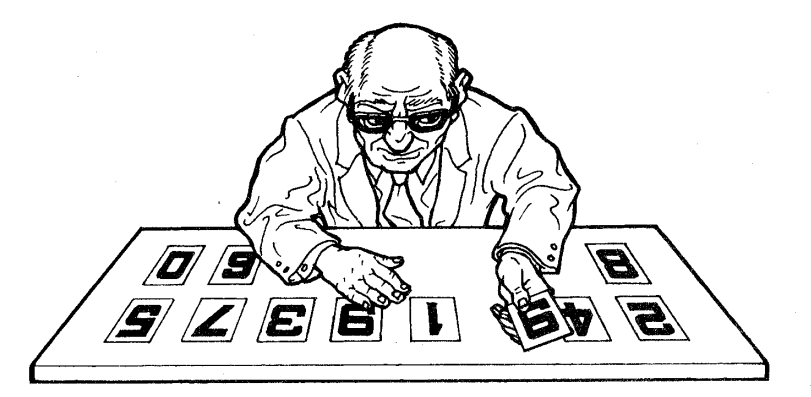
\includegraphics[scale=0.8]{./estáticos/ordenacionArrays.png}
\caption{Ordenación de arreglos}
\end{figure}

La principal condición a imponer a los métodos de ordenación de arreglos es la utilización económica de la memoria disponible. Esto implica que las permutaciones de items, con vistas a su ordenación, deben realizarse utilizando el espacio ocupado por el arreglo y que los métodos que transportan artículos de un array $a$ hacia un array resultado $b$ son intrínsecamente de menor interés.

\section{Ordenación por selección}
Este método se basa en los siguientes principios:
\begin{enumerate}
    \item Seleccionar el menor elemento.
    \item Intercambiarlo con el primer elemento.
\end{enumerate}
Y luego se repite el proceso con el resto del arreglo, es decir, se selecciona el menor elemento del subarreglo restante y se intercambia con el segundo elemento, y así sucesivamente.
\newpage
\begin{figure}[h]
\centering
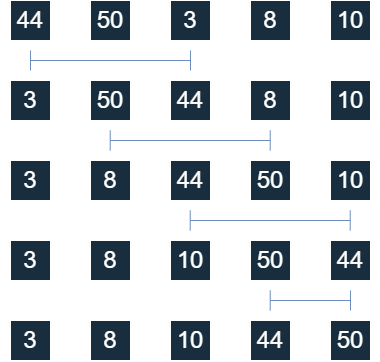
\includegraphics[scale=0.5]{./estáticos/ordSeleccion.png}
\caption{Ejemplo de proceso de ordenación por selección}
\end{figure}

Para el algoritmo de ordenación por selección, se ha desarrollado un procedimiento \texttt{selection\_sort} que recibe un arreglo de tamaño $n$ y lo ordena. El procedimiento \texttt{selection\_sort} utiliza dos funciones auxiliares: \texttt{min\_pos\_from} y \texttt{swap}. La función \texttt{min\_pos\_from} recibe un arreglo y una posición, y retorna la posición del menor elemento a partir de la posición dada. La función \texttt{swap} recibe un arreglo y dos posiciones, e intercambia los elementos en dichas posiciones. Se pueden marcar las siguientes observaciones:

\begin{itemize}
    \item \texttt{selection\_sort} utiliza un ciclo \texttt{for} que recorre el arreglo desde la primera posición hasta la última. En cada iteración, se busca el menor elemento a partir de la posición actual y se intercambia con el elemento en la posición actual,
    \item se encuentra una llamada a la función \texttt{min\_pos\_from} que recibe el arreglo y la posición actual, y retorna la posición del menor elemento a partir de la posición actual,
    \item y se recibe tambien una llamada al procedimiento \texttt{swap} que recibe el arreglo y las posiciones actual y la posición del menor elemento, e intercambia los elementos en dichas posiciones,
    \item encontramos una \textbf{comparación} entre elementos de un arreglo, y una \textbf{asignación} de elementos de un arreglo,
    \item la operación que mas se repite es la comparación de elementos de un arreglo, y toda operación se repite a lo sumo de manera proporcional a esa,
    \item como la celda de un arreglo es constante, su costo no depende de cual es la celda o del tamaño del arreglo, por lo que el costo de la operación es constante.
\end{itemize}

\subsection{Código}

\begin{codebox}{Código 25}
\footnotesize Ordenación por selección
\tcblower
\begin{pascallike}
proc selection_sort (in/out a: array[1..n] of T)
    var minp: nat
    for i := 1 to n do
        minp := min_pos_from(a, i)
        swap(a, i, minp) 
    od
end proc

fun min_pos_from (a: array[1..n] of T, i: nat) ret minp: nat
    minp := i
    for j:= i+1 to n do 
        if a[j] < a[minp] then 
            minp:= j 
        fi
    od
end fun

proc swap (in/out a: array[1..n] of T, in i, j: nat)
    var temp: T
    temp := a[i]
    a[i] := a[j]
    a[j] := temp
end proc
\end{pascallike}
\end{codebox}

\subsection{Análisis de complejidad}
\begin{itemize}
    \item Al llamar a la función \texttt{min\_pos\_from} se realiza una cantidad de operaciones proporcional a $n-i$,
    \item \texttt{selection\_sort} llama a \texttt{min\_pos\_from(a,i)} para $i=1,2,\ldots,n-1$,
    \item por lo tanto, en total son $(n-1) + (n-2) + \ldots + 1 = \frac{n(n-1)}{2}$ comparaciones.
\end{itemize}

\section{Ordenación por inserción}
Este método se basa en los siguientes principios:
\begin{enumerate}
    \item Seleccionar el primer elemento del arreglo.
    \item Insertarlo en la posición correcta.
\end{enumerate}
Y luego se repite el proceso con el resto del arreglo, es decir, se selecciona el siguiente elemento y se inserta en la posición correcta.

\newpage
\begin{figure}[h]
\centering
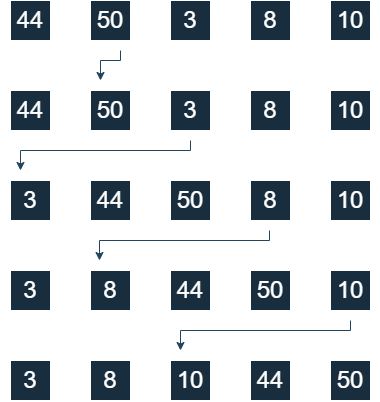
\includegraphics[scale=0.5]{./estáticos/ordInsercion.png}
\caption{Ejemplo de proceso de ordenación por inserción}
\end{figure}

Para el algoritmo de ordenación por inserción, se ha desarrollado un procedimiento \texttt{insertion\_sort} que recibe un arreglo de tamaño $n$ y lo ordena. El procedimiento \texttt{insertion\_sort} utiliza un procedimiento auxiliar \texttt{insert}. El procedimiento \texttt{insert} recibe un arreglo y una posición, y mueve el elemento en la posición dada a la posición correcta. 

\begin{itemize}
    \item \texttt{insertion\_sort} utiliza un ciclo \texttt{for} que recorre el arreglo desde la segunda posición hasta la última. En cada iteración, se llama al procedimiento \texttt{insert} que recibe el arreglo y la posición actual, y mueve el elemento en la posición actual a la posición correcta,
    \item se encuentra una llamada al procedimiento \texttt{insert} que recibe el arreglo y la posición actual, y mueve el elemento en la posición actual a la posición correcta.
\end{itemize}

\subsection{Código}

\begin{codebox}{Código 26}
\footnotesize Ordenación por inserción
\tcblower
\begin{pascallike}
proc insertion_sort (in/out a: array[1..n] of T)
    for i:= 2 to n do
        insert(a,i)
    od
end proc
proc insert (in/out a: array[1..n] of T, in i: nat)
    var j: nat
    j:= i
    do j > 1 && a[j] < a[j - 1] -> 
        swap(a,j-1,j)
        j:= j-1
    od
end proc
\end{pascallike}
\end{codebox}

\subsection{Análisis de complejidad}
\begin{itemize}
    \item En el peor caso, el arreglo está ordenado en forma inversa, por lo que se deben realizar $i-1$ comparaciones en la posición $i$,
    \item \texttt{insertion\_sort} llama a \texttt{insert(a,i)} para $i=2,3,\ldots,n$,
    \item por lo tanto, en total son $1 + 2 + \ldots + n-1 = \frac{n(n-1)}{2}$ comparaciones.
\end{itemize}